\documentclass[tikz]{standalone}
\usetikzlibrary{arrows.meta}

%usepackage[utopia]{mathdesign}
\usepackage[]{tgheros}
\renewcommand{\familydefault}{\sfdefault}
\usepackage{arevmath}
\usepackage[italic]{mathastext}
\usepackage[T1]{fontenc}

\begin{document}
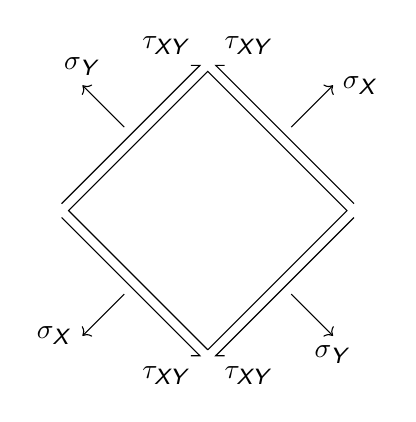
\begin{tikzpicture}[scale=2.5]

    \draw[rotate=45] (0,0) -- (0,1) -- (1,1) -- (1,0) -- (0,0);
    
    
    \draw[->, rotate=45] (-0.1,0.5) -- (-0.4,0.5) node[left]{$\sigma_X$};
    \draw[->, rotate=45] (1.1,0.5) -- (1.4,0.5) node[right]{$\sigma_X$};
    \draw[->, rotate=45] (0.5,1.1) -- (0.5,1.4) node[above]{$\sigma_Y$};
    \draw[->, rotate=45] (0.5,-0.1) -- (0.5,-0.4) node[below]{$\sigma_Y$};
    
    \draw[{Straight Barb[left]}-, rotate=45] (0.0,-0.05) -- (1.0,-0.05) node[pos=0.0, anchor=north west]{$\tau_{XY}$};
    \draw[-{Straight Barb[left]}, rotate=45] (0.0,1.05) -- (1.0,1.05) node[pos=1.0, anchor=south east]{$\tau_{XY}$};
    
    \draw[{Straight Barb[right]}-, rotate=45] (-0.05,0.0) -- (-0.05,1.0) node[pos=0.0, anchor=north east]{$\tau_{XY}$};
    \draw[-{Straight Barb[right]}, rotate=45] (1.05,0.0) -- (1.05,1.0) node[pos=1.0, anchor=south west]{$\tau_{XY}$};

\end{tikzpicture}
\end{document}